\question[6] (5分)一细绳跨过悬挂的定滑轮,两端分别系有小球A和B,如图所示。一实验小组用此装置测量小球B运动的加速度。
\begin{center}
    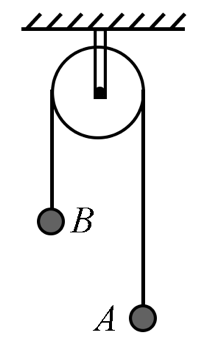
\includegraphics[]{img/image5.png}
    \end{center}
令两小球静止,细绳拉紧,然后释放小球,测得小球B释放时的高度$h_0=0.590m,$下降一段距离后的高度$h=0.100m;$由$h_0$下降至h所用的时间$T=0.730s$。由此求得小球B加速度的大小为a=\key{1.84}$m/s^2($保留3位有效数字)。

从实验室提供的数据得知,小球A、B的质量分别为$100.0g$和$150.0g,$当地重力加速度大小为$g=9.80m/s^2.$根据牛顿第二定律计算可得小球B加速度的大小为$a^\prime=$\key{1.96}$m/s^2($保留3位有效数字)。

可以看出$,a^\prime$与a有明显差异,除实验中的偶然误差外,写出一条可能产生这一结果的原因:\key{滑轮的轴不光滑(或滑轮有质量)}。


\question[6] $(10$分)某同学要研究一小灯泡$L(3.6V,0.30A)$的伏安特性。所用器材有:电流表$A_1($量程$200mA,$内阻$R_g1=10.0Ω),$电流表$A_2($量程$500mA,$内阻$R_g2=1.0Ω)$、定值电阻$R_0($阻值$R0=10.0Ω)$、滑动变阻器$R_1($最大阻值$10Ω)$、电源E(电动势$4.5V,$内阻很小)、开关S和若干导线.该同学设计的电路如图(a)所示。

(1)根据图$(a),$在图(b)的实物图中画出连线。
\begin{center}
    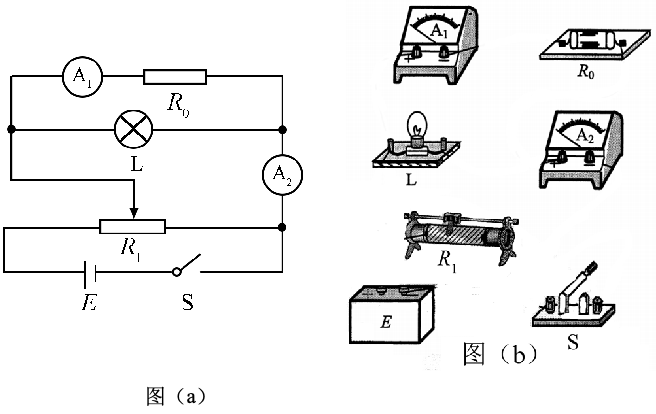
\includegraphics[]{img/image6.png}
    \end{center}
(2)若$I_1$、$I_2$分别为流过电流表$A_1$和$A_2$的电流,利用$I_1$、$I_2$、$R_g1$和$R_0$写出:小灯泡两端的电压U=\key{$I_1(R_{g1}+R_0)$}流过小灯泡的电流I=\key{$I_2-I_1$}。为保证小灯泡的安全$,I_1$不能超过\key{180}mA。

(3)实验时,调节滑动变阻器,使开关闭合后两电流表的示数为零。逐次改变滑动变阻器滑片位置并读取相应的$I_1$和$I_2$。所得实验数据在下表中给出。
\begin{table}[h]
    \begin{center}
        \begin{tabular}{|l|l|l|l|l|l|l|}
        \hline
        $I_1/mA$ & 32  & 55  & 85  & 125 & 144 & 173 \\ \hline
        $I_2/mA$ & 171 & 229 & 299 & 379 & 424 & 470 \\ \hline
        \end{tabular}
    \end{center}
\end{table}


根据实验数据可算得,当$I_1=173mA$时,灯丝电阻R=\key{11.6}Ω(保留1位小数)

(4)如果用另一个电阻替代定值电阻$R_0,$其他不变,为了能够测量完整的伏安特性曲线,所用电阻的阻值不能小于\key{8.0}Ω(保留1位小数)。


\question[6] $(12$分)如图,在$0≤x≤h,–∞<y<+∞$区域中存在方向垂直于纸面的匀强磁场,磁感应强度B的大小可调,方向不变。一质量为m,电荷量为$q(q>0)$的粒子以速度$v_0$从磁场区域左侧沿x轴进入磁场,不计重力。
\begin{center}
    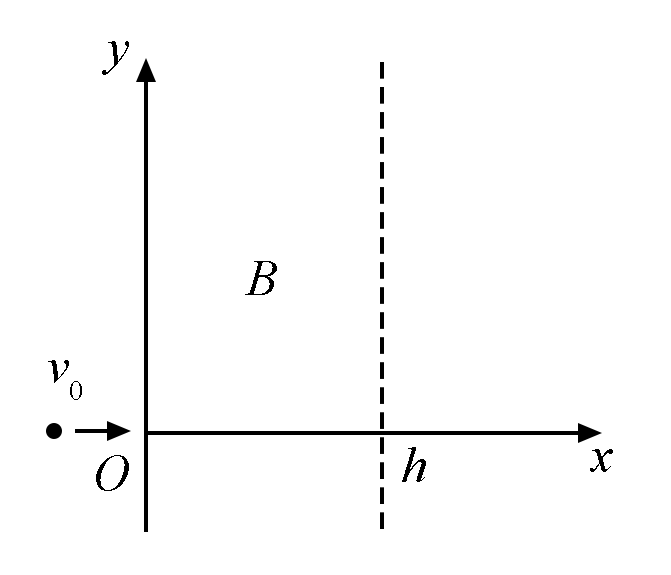
\includegraphics[]{img/image7.png}
    \end{center}
(1)若粒子经磁场偏转后穿过y轴正半轴离开磁场,分析说明磁场的方向,并求在这种情况下磁感应强度的最小值$B_m;$

(2)如果磁感应强度大小为$\frac{B_{m}}{2},$粒子将通过虚线所示边界上的一点离开磁场.求粒子在该点的运动方向与x轴正方向的夹角及该点到x轴的距离。
\begin{solution}{4cm}
(1)由题意 , 粒子刚进入磁场时应受到方向向上的洛伦兹力 , 因此磁场方向垂直于纸面向里 .设粒子进入磁场中做圆周运动的半径为 R , 根据洛伦兹力公式和圆周运动规律 , 有 

$qv_{0}B=m \frac{V_{0}^{2}}{R}$\ding{172}

由此可得 
$R= \frac{mv_{0}}{qB}$ \ding{173}

粒子穿过 y 轴正半轴离开磁场 , 其在磁场中做圆周运动的圆心在 y 轴正半轴上 , 半径应满足

$R≤ h$ \ding{174}

由题意 , 当磁感应强度大小为 $B _m$ 时 , 粒子的运动半径最大 , 由此得 
$B_{m}= \frac{mv_{0}}{qh}$ \ding{175}

(2)若磁感应强度大小为  $\frac{B_{m}}{2}$  , 粒子做圆周运动的圆心仍在 y 轴正半轴上 , 由\ding{173}\ding{175}式可得 , 此时圆弧半径为 $R^\prime= 2 h$ \ding{176}

粒子会穿过图中 P 点离开磁场 , 运动轨迹如图所示 . 设粒子在 P 点的运动方向与 x 轴正方向的夹角为α ,
\begin{center}
    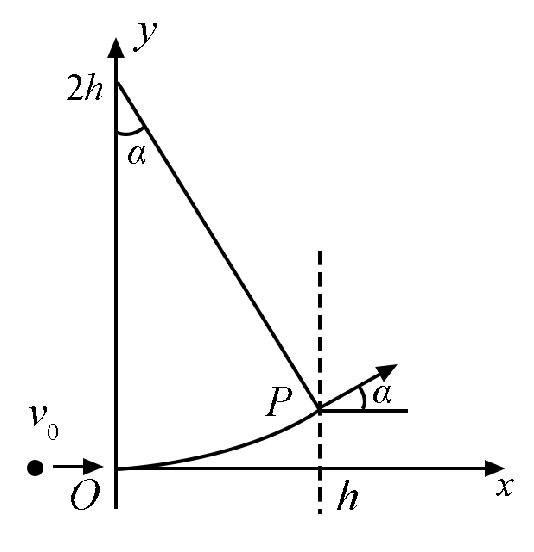
\includegraphics[width=3cm]{img/imageA1.png}
\end{center}  
由几何关系 
$\sin \alpha = \frac{h}{2h}= \frac{1}{2}$ \ding{177}

即
$\alpha = \frac{ \pi }{6}$\ding{178}

由几何关系可得 , P 点与 x 轴的距离为
$y = 2 h ( 1- cos α )$ \ding{179}

联立\ding{178}\ding{179} 式得 
$y=(2- \sqrt{3})h$\ding{180}
\end{solution}

\question[6] $(20$分)如图,一竖直圆管质量为M,下端距水平地面的高度为H,顶端塞有一质量为m的小球。圆管由静止自由下落,与地面发生多次弹性碰撞,且每次碰撞时间均极短;在运动过程中,管始终保持竖直。已知$M=4m,$球和管之间的滑动摩擦力大小为$4mg,g$为重力加速度的大小,不计空气阻力。

(1)求管第一次与地面碰撞后的瞬间,管和球各自的加速度大小;

(2)管第一次落地弹起后,在上升过程中球没有从管中滑出,求管上升的最大高度;

(3)管第二次落地弹起的上升过程中,球仍没有从管中滑出,求圆管长度应满足的条件。
\begin{center}
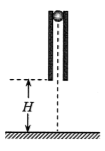
\includegraphics[]{img/image8.png}
\end{center}
\begin{solution}{4cm}
(1)管第一次落地弹起的瞬间 , 小球仍然向下运动 . 设此时管的加速度大小为 $a _1$ , 方向向下 ; 球的加速度大小为 $a _2$ , 方向向上 ; 球与管之间的摩擦力大小为 f , 由牛顿运动定律有

$Ma _1 = Mg + f$ \ding{172}
$ma _2 = f - mg$ \ding{173}

联立\ding{172}\ding{173}式并代入题给数据 , 得
$a _1 = 2 g ,  a_{2}=3g$\ding{174} 

(2)管第一次碰地前与球的速度大小相同 . 由运动学公式 , 碰地前瞬间它们的速度大小均为

$v_{0}= \sqrt{2gH}$ \ding{175}

方向均向下 . 管弹起的瞬间 , 管的速度反向 , 球的速度方向依然向下 .

设自弹起时经过时间 $t _1$ , 管与小球的速度刚好相同 . 取向上为正方向 , 由运动学公式

$v_0- a _1t _1 = - v _0+ a _2 t_1$ \ding{176}

联立\ding{174}\ding{175}\ding{176}式得 
$t_{1}= \frac{2}{5} \sqrt{ \frac{2H}{g}}$ 

设此时管下端的高度为 $h _1$ , 速度为 v . 由运动学公式可得

$h_{1}=v_{0}t_{1}- \frac{1}{2}a_{1}t_{1}^{2}$ \ding{178}
$v = v _0- a _1t _1$ \ding{179}

由\ding{174}\ding{175}\ding{177}\ding{179}式可判断此时 $v > 0$ . 此后 , 管与小球将以加速度 g 减速上升 $h _2$ , 到达最高点 . 由运动学公式有  
$h_{2}= \frac{v^{2}}{2g}$ \ding{180}

设管第一次落地弹起后上升的最大高度为 $H _1$ , 则$H _1 = h _1+ h _2$ \circled{10}

联立\ding{174}\ding{175}\ding{177}\ding{178}\ding{179}\ding{180}式可得 $H_{1}= \frac{13}{25}H$ \circled{11}

(3)设第一次弹起过程中球相对管的位移为 $x _1$ . 在管开始下落到上升 $H _1$ 这一过程中 , 由动能定理有
$Mg ( H - H _1 ) + mg ( H - H _1+ x _1 ) -4 mgx1 = 0$ \circled{12} 

联立\circled{11}\circled{12}式并代入题给数据得 $x_{1}= \frac{4}{5}H_{1}$ \circled{13}

同理可推得 , 管与球从再次下落到第二次弹起至最高点的过程中 , 球与管的相对位移 $x _2 $为

$ x_{2}= \frac{4}{5}H_{1}$\circled{14} 

设圆管长度为 L . 管第二次落地弹起后的上升过程中 , 球不会滑出管外的条件是
$x _1+ x2 ≤ L$\circled{15}
联立\circled{11}\circled{13}\circled{14}\circled{15}式 , L 应满足条件为 $L \geqslant \frac{152}{125}H$\circled{16}

\end{solution}
(二)选考题:共 45 分。请考生从 2 道物理题、2 道化学题、2 道生物题中每科任选一题作答。如果多做, 则\textcolor{red}{每科}按所做的第一题计分。
\question[6] [物理——选修$3-3](15$分)

(1)(5分)下列关于能量转换过程的叙述,违背热力学第一定律的有\key{B},不违背热力学第一定律、但违背热力学第二定律的有\key{C}。(填正确答案标号)

A.汽车通过燃烧汽油获得动力并向空气中散热

B.冷水倒入保温杯后,冷水和杯子的温度都变得更低

C.某新型热机工作时将从高温热源吸收的热量全部转化为功,而不产生其他影响

D.冰箱的制冷机工作时从箱内低温环境中提取热量散发到温度较高的室内

(2)$(10$分)潜水钟是一种水下救生设备,它是一个底部开口、上部封闭的容器,外形与钟相似。潜水钟在水下时其内部上方空间里存有空气,以满足潜水员水下避险的需要。为计算方便,将潜水钟简化为截面积为S、高度为h、开口向下的圆筒;工作母船将潜水钟由水面上方开口向下吊放至深度为H的水下,如图所示。已知水的密度为ρ,重力加速度大小为g,大气压强为$po,H≫h,$忽略温度的变化和水密度随深度的变化。

(i)求进入圆筒内水的高度l;

(ii)保持H不变,压入空气使筒内的水全部排出,求压入的空气在其压强为$p_0$时的体积。
\begin{center}
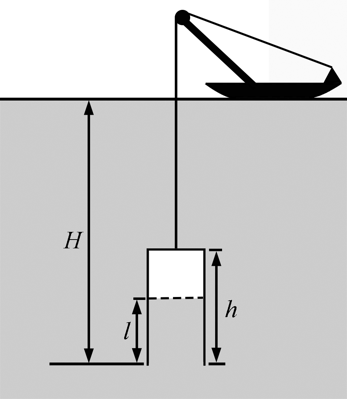
\includegraphics[]{img/image9.png}
\end{center}
\begin{solution}{4cm}
(i)
设潜水钟在水面上方时和放入水下后筒内气体的体积分别为 $V _0$ 和 $V _1$ , 放入水下后筒内气体的压强为 $p _1$ , 由玻意耳定律和题给条件有

$p _1V _1 = p_0V _0$

$V_0 = hS$

$V _1 = ( h - l ) S$

$p _1 = p_0 + ρ g ( H - l )$ \ding{175}

联立以上各式并考虑到 $H ≫ h > l$ , 解得 
$l= \frac{ \rho gH}{p_{0}+ \rho gH}h $

(ii)
设水全部排出后筒内气体的压强为 $p_2$ ; 此时筒内气体的体积为 $V _0$ , 这些气体在其压强为 $p _0$ 时的体积为 $V _3$ , 由玻意耳定律有

$p _2 V _0 = p_0V _3$

其中 
$p _2 = p _0+ ρ gH $ \ding{178}

设需压入筒内的气体体积为 V , 依题意$V = V _3- V _0$
联立\ding{173}\ding{177}\ding{178}⑧式得 

$V= \frac{ \rho gSHh}{p_{0}}$ ⑨ 
\end{solution}
\question[6] [物理--选修$3-4](15$分)

(1)(5分)用一个摆长为$80.0cm$的单摆做实验,要求摆动的最大角度小于$5°,$则开始时将摆球拉离平衡位置的距离应不超过\key{6.9}$cm($保留1位小数)。(提示:单摆被拉开小角度的情况下,所求的距离约等于摆球沿圆弧移动的路程。)

某同学想设计一个新单摆,要求新单摆摆动10个周期的时间与原单摆摆动11个周期的时间相等。新单摆的摆长应该取为\key{96.8}cm。

(2)$(10$分)直角棱镜的折射率$n=1.5,$其横截面如图所示,图中$∠C=90^∘,∠A=30$。截面内一细束与BC边平行的光线,从棱镜AB边上的D点射入,经折射后射到BC边上。
\begin{center}
    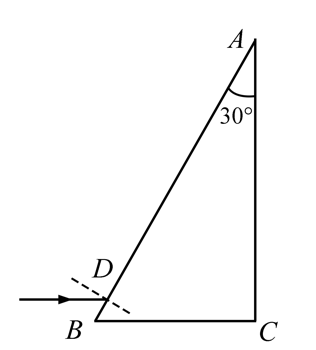
\includegraphics[]{img/image10.png}
    \end{center}
(i)光线在BC边上是否会发生全反射?说明理由;

(ii)不考虑多次反射,求从AC边射出的光线与最初的入射光线夹角的正弦值。
\begin{solution}{4cm}
(i)
如图 , 设光线在 D 点的入射角为 i , 折射角为 r . 折射光线射到 BC 边上的 E 点 . 设光线在 E 点的入射角为 θ , 由几何关系 , 有
\begin{center}
    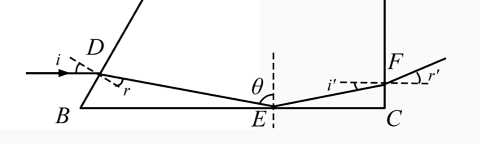
\includegraphics[]{img/imgageA2.png}
\end{center}
$θ = 90 ^∘ - ( 30^∘ - r ) > 60^∘$ \ding{172}

根据题给数据得 $\sin \theta > \sin 60^{ \circ }> \frac{1}{n}$ \ding{173}

即 θ大于全反射临界角 , 因此光线在 E 点发生全反射 .   

(ii)
设光线在 AC 边上的 F 点射出棱镜 , 光线的入射角为 $i^\prime$ , 折射角为 $r^\prime$ , 由几何关系、反射定律及折射定律 , 有

$i = 30 ^∘$\ding{174}

$i^\prime = 90^∘ - θ$\ding{175}

$sin i = nsinr$ \ding{176}

$nsini^\prime = sinr ^\prime$ \ding{177}

联立\ding{172}\ding{174}\ding{175}\ding{176}\ding{177}式并代入题给数据 , 得 

$\sin r^{ \prime }= \frac{2 \sqrt{2}- \sqrt{3}}{4} $\ding{178}

由几何关系 , $r^\prime$即 AC 边射出的光线与最初的入射光线的夹角 .
\end{solution}

